%! Author = Aleksandr.Avdiushenko
%! Date = 17/02/2025

\documentclass{article}
\usepackage{tikz}
\usepackage{pgfplots}
\usetikzlibrary{positioning, decorations.pathreplacing}

\begin{document}

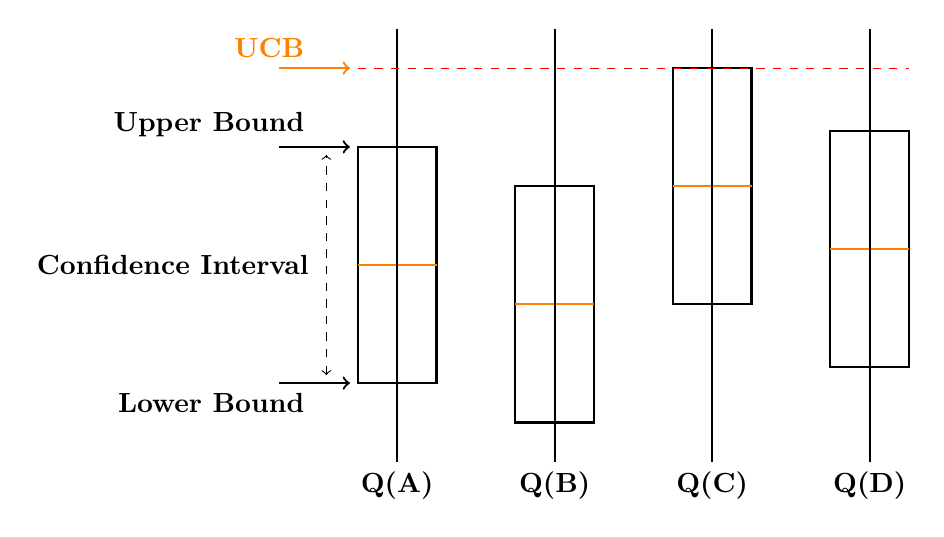
\begin{tikzpicture}
    % Define styles
    \tikzstyle{box} = [draw, thick, minimum width=1cm, minimum height=3cm]
    \tikzstyle{median} = [draw, thick, orange]
    \tikzstyle{whisker} = [draw, thick]

    % Draw boxplots
    \def\x{0}
    \def\xlabel{A}
    \node[box] (box\x) at (\x,2) {};
    \draw[median] (
        \x-0.5,2) -- (\x+0.5,2);
    \draw[whisker] (
        \x, -0.5) -- (\x, 5);

    \def\x{2}
    \def\xlabel{B}
    \node[box] (box\x) at (\x,1.5) {};
    \draw[median] (
        \x-0.5,1.5) -- (\x+0.5,1.5);
    \draw[whisker] (
        \x, -0.5) -- (\x, 5);

    \def\x{4}
    \def\xlabel{C}
    \node[box] (box\x) at (\x,3) {};
    \draw[median] (
        \x-0.5,3) -- (\x+0.5,3);
    \draw[whisker] (
        \x, -0.5) -- (\x, 5);

    \def\x{6}
    \def\xlabel{D}
    \node[box] (box\x) at (\x,2.2) {};
    \draw[median] (
        \x-0.5,2.2) -- (\x+0.5,2.2);
    \draw[whisker] (
        \x, -0.5) -- (\x, 5);

    % Special annotations for Q(A)
    \draw[dashed, <->] (-0.9,0.6) -- (-0.9,3.4);
    \node[anchor=west] at (-4.7,2) {\textbf{Confidence Interval}};

    \draw[->, thick] (-1.5,3.5) -- (-0.6,3.5) node[midway, above left] {\textbf{Upper Bound}};
    \draw[->, thick] (-1.5,0.5) -- (-0.6,0.5) node[midway, below left] {\textbf{Lower Bound}};

    % Upper bound arrow and dashed line
    \draw[thick, ->, orange] (-1.5,4.5) -- (-0.6,4.5) node[midway, above left] {\textbf{UCB}};
    \draw[dashed, red] (-0.5,4.5) -- (6.5,4.5);

    % Labels for boxplots
    \foreach \x/\label in {0/Q(A), 2/Q(B), 4/Q(C), 6/Q(D)} {
        \node[below] at (\x, -0.5) {\textbf{\label}};
    }
\end{tikzpicture}

\end{document}
